Intel's Software Guard Extensions (SGX) is the latest iteration in a long line
of trusted computing (Figure~\ref{fig:trusted_computing}) designs, which aim to
solve the secure remote computation problem by leveraging trusted hardware in
the remote computer. The trusted hardware establishes a secure container, and
the remote computation service user uploads the desired computation and data
into the secure container. The trusted hardware protects the data's privacy
and integrity while the computation is being performed on it.

\begin{figure}[hbt]
  \centering
  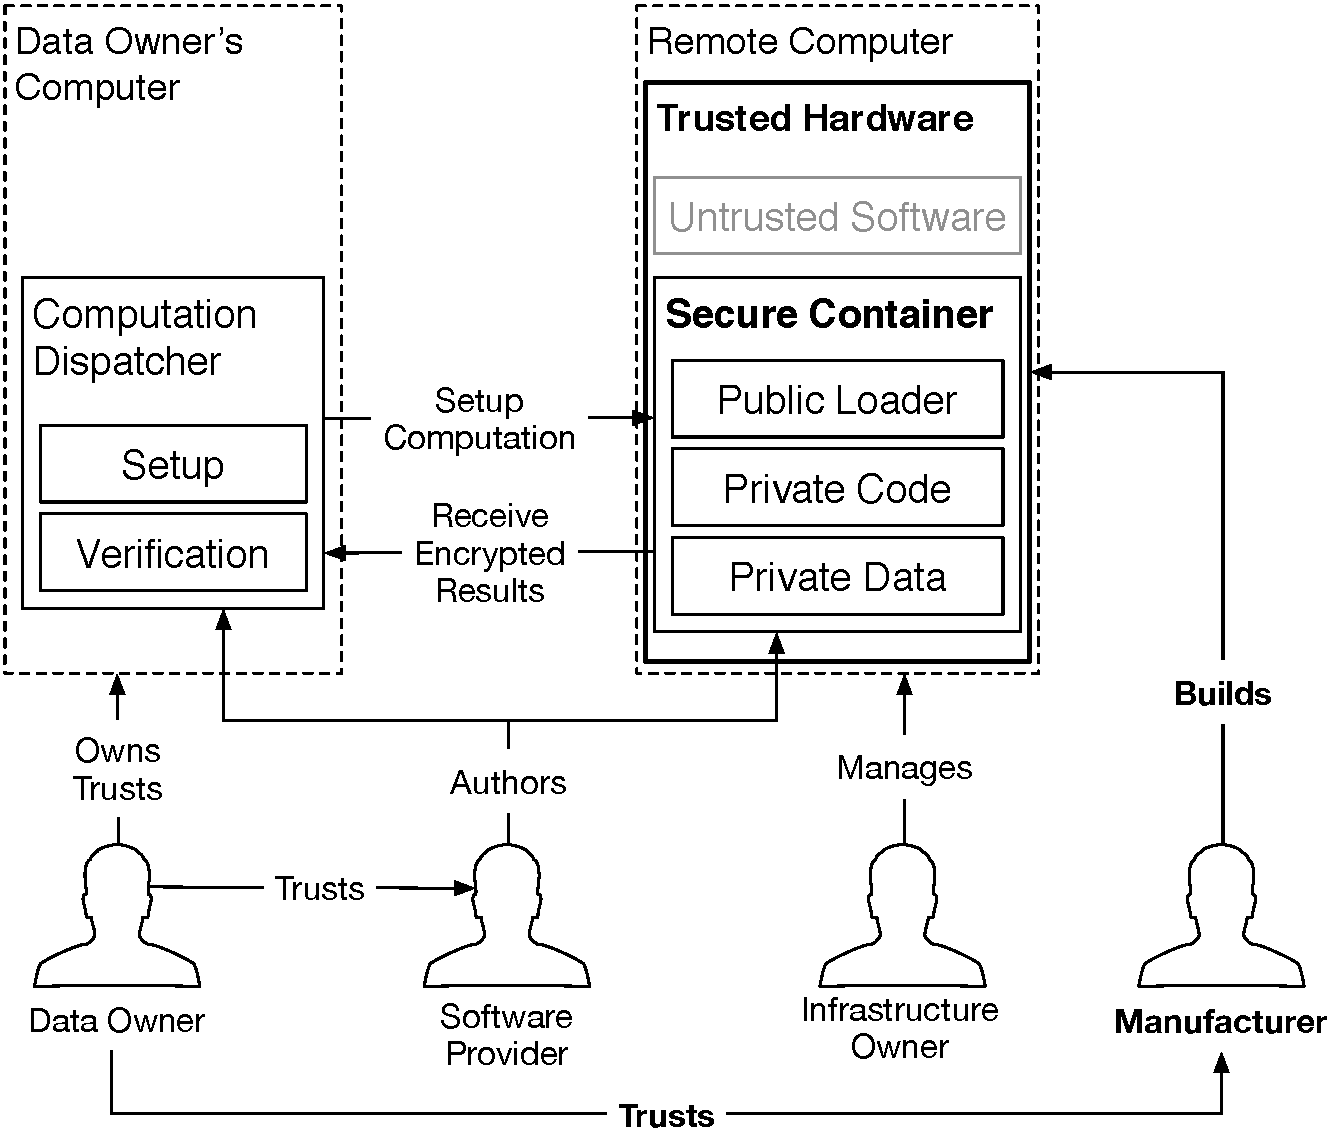
\includegraphics[width=85mm]{figures/trusted_computing.pdf}
  \caption{
    Trusted computing. The user trusts the manufacturer of a piece of hardware
    in the remote computer, and entrusts her data to a secure container hosted
    by the secure hardware.
  }
  \label{fig:trusted_computing}
\end{figure}

SGX relies on \textit{software attestation}, like its predecessors, the
TPM~\cite{grawrock2003tpm} and TXT~\cite{grawrock2009txt}. Attestation
(Figure~\ref{fig:generic_attestation}) proves to a user that she is
communicating with a specific piece of software running in a secure container
hosted by the trusted hardware. The proof is a cryptographic signature that
certifies the hash of the secure container's contents. It follows that the
remote computer's owner can load any software in a secure container, but the
remote computation service user will refuse to load her data into a secure
container whose contents' hash does not match the expected value.

\begin{figure}[hbt]
  \centering
  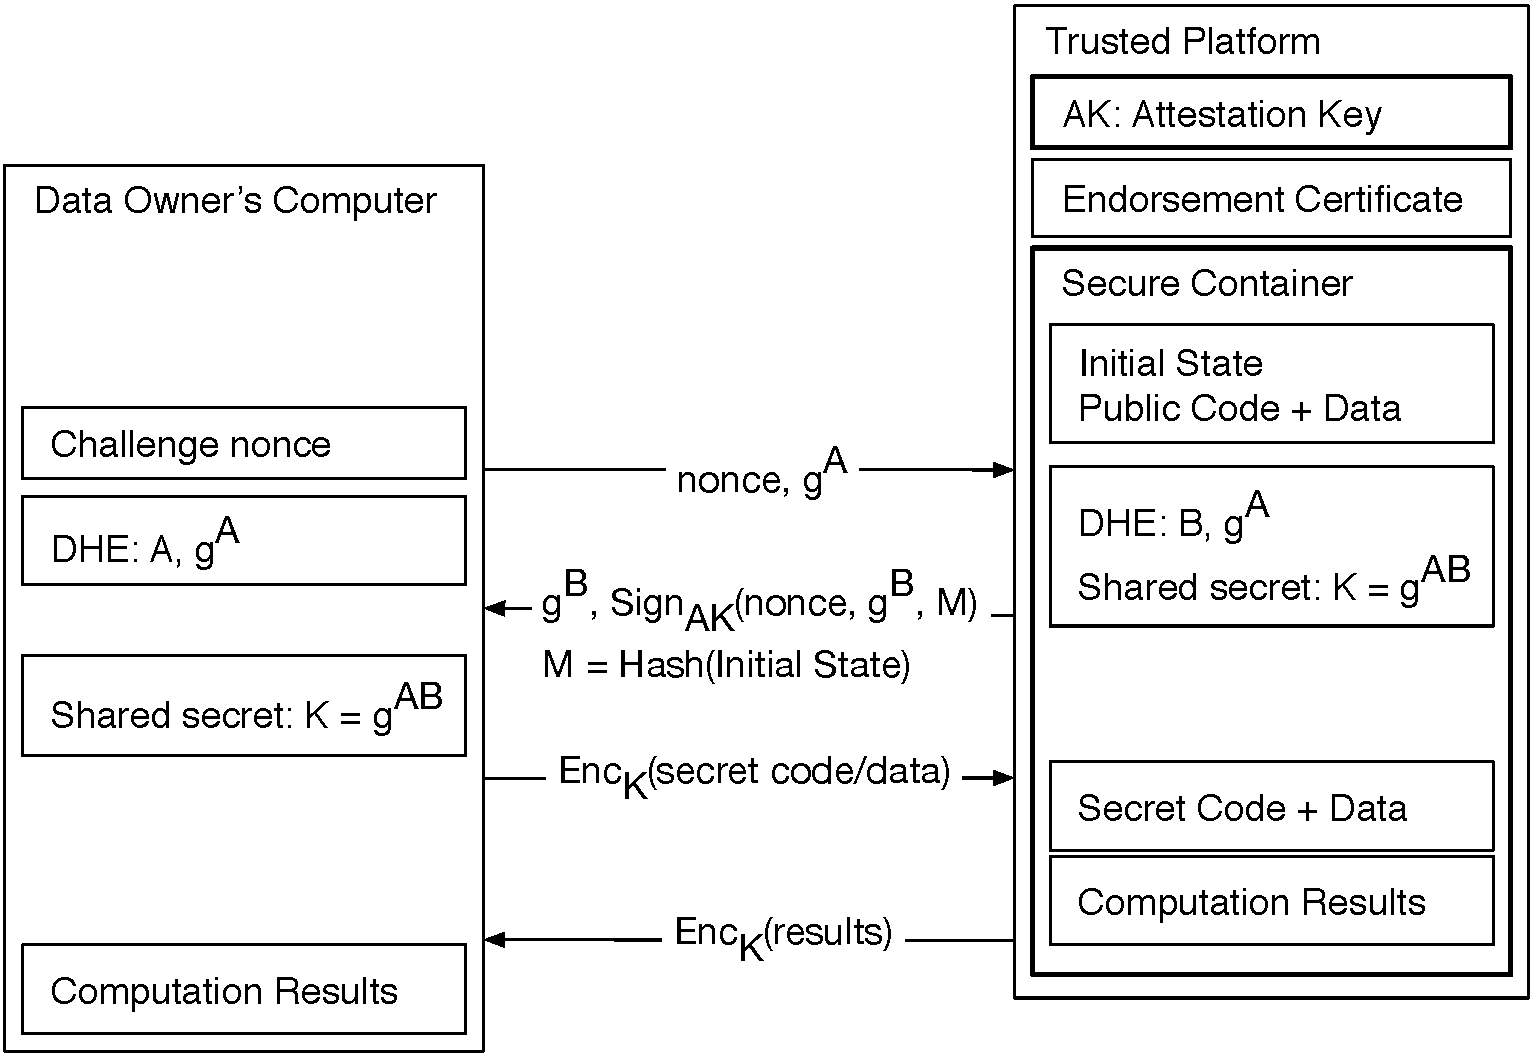
\includegraphics[width=87mm]{figures/generic_attestation.pdf}
  \caption{
    Software attestation proves to a remote computer that it is communicating
    with a specific secure container hosted by a trusted platform. The proof is
    an attestation signature produced by the platform's secret attestation key.
    The signature covers the container's initial state, a challenge nonce
    produced by the remote computer, and a message produced by the container.
  }
  \label{fig:generic_attestation}
\end{figure}

The remote computation service user verifies the \textit{attestation key} used
to produce the signature against an \textit{endorsement certificate} created by
the trusted hardware's manufacturer. The certificate states that the
attestation key is only known to the trusted hardware, and only used for the
purpose of attestation.
